\begin{frame}{caches}
    \begin{itemize}
    \item caches --- fast memory that holds\\
        \myemph{recently accessed values from main memory} and \\
        \myemph{values near recently accessed values from main memory}
    \item idea: program thinks it accesses main memory\ldots \\
        but most accesses take `shortcut' to cache
    \end{itemize} 
\end{frame}

\begin{frame}[fragile,label=observeCaches]{observing caches}
\lstset{
    language=C++,style=smaller
}
\begin{lstlisting}
unsigned run(int count) {
    unsigned index = 1;
    for (unsigned j = 0; j < count; ++j) {
        // use array @ index to find next index
        // prevents parallel accesses to cache/memory
        index = array[index];
    }
    return index;
}

// setup to access array with bad spatial locality
// size is the approx. # elements to access
void setup(int size) {
    for (int i = 0; i < size; ++i)
        order[i] = i;
    randomlyShuffle(order, size);
    for (int i = 0; i < size - 1; ++i) {
        /* order[i] should point to order[i+1] */
        array[order[i]] = order[(i + 1) % size];
    }
    array[index] = 0;
}
\end{lstlisting}
\end{frame}

\begin{frame}{observing caches}
    \vspace{-1cm}
    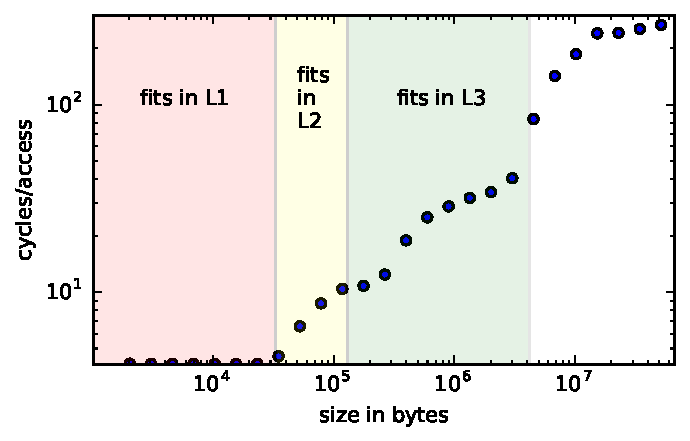
\includegraphics[width=\textwidth]{size-v-cycles}
\end{frame} 
